% Source - https://tex.stackexchange.com/a/133670

\documentclass[tikz]{standalone}
\usetikzlibrary{nfold}
\makeatletter
\tikzset{
    offset/.code=\tikz@addmode{
        \pgfgetpath\tikz@temp
        \pgfsetpath\pgfutil@empty
        \pgfoffsetpath\tikz@temp{#1}
    }
}
\makeatother
\begin{document}
\tikz[nodes={circle, fill, inner sep=+1.5pt}]
\draw[preaction={rounded corners, offset=10pt, fill=gray}]
    (-2, 3) node (A) {}
    ( 3, 4) node (B) {}
    ( 2,-1) node (C) {}
    (-2,-4) node (D) {}
    (-4, 0) node (E) {}
    plot[sharp cycle, samples at={A, ..., E}] (\x);

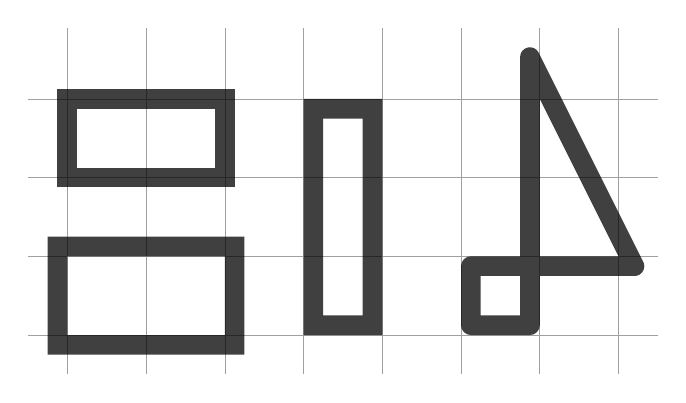
\begin{tikzpicture}[line width=.25cm, opacity=.75]
    \draw[help lines] (-.5, -.5) grid (7.5, 3.9);
    \draw  (0,2) rectangle (2,3);
    \draw[offset=.5\pgflinewidth]  (0,0) rectangle (2,1);
    \draw[offset=-.5\pgflinewidth] (3,0) rectangle (4,3);
    \path[xshift=5cm, offset=.5\pgflinewidth, draw, line join=round] (0,0) -| (1,3) -- (2,1) -- (0,1) -- cycle;
\end{tikzpicture}

\tikz[line width=.2cm]
  \path[
        postaction={draw=blue,                     offset=+ .5\pgflinewidth},
        postaction={draw=red, fill=green!50!black, offset=+-.5\pgflinewidth},
        bend left
    ] (0,0) to ++(30:2) to ++ (-60:2) to ++(-150:2) to cycle;
\end{document}
